% 2020 新高考Ⅱ卷 16：某零件的截面（1 单位 = 1 cm，整图 scale=0.75）
% 绘制依据：源 PDF 原图逐像素核对。矩形 DEFG：D(0,2)、E(0,0)、F(12,0)、G(12,2)，
% ED/EF/FG 实线、DG 虚线；外轮廓弧圆心 O(5,5)、半径 R=2√2，弧顶 (5,7.83)；
% A(7,7) 与 B(2.172,5) 为切点（GA 与弧相切于 A、竖直的 BC 与弧相切于 B），
% C(2.172,2) 是 B 在 DG 上的垂足，H(9,5) 在直线 GA 上且与 B、O 共线于 y=5。
% 实线闭合轮廓：E→F→G→A→（弧 45°逆时针经弧顶到 180°）→B→C→D→E。
% 虚线四条：B–O–H、D–C…G、过 O 的竖直中心线（弧顶落到 (5,2)）、线段 D–O。
% 阴影 gray!25：弧 B→A + 线段 A→H + 线段 H→B 围成的区域；半径 1 的圆孔整体留白
% （先填灰、再以白色填圆，故 BH 以下不着色），中心线穿孔而过。
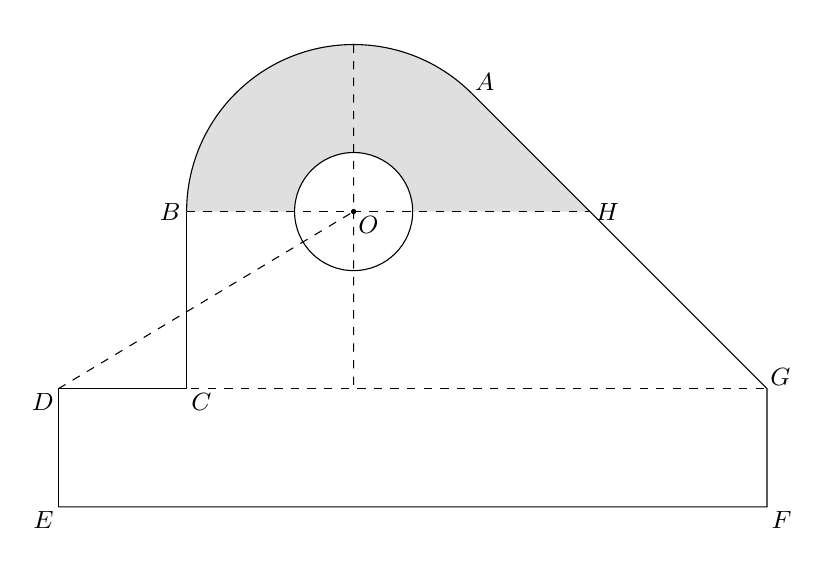
\begin{tikzpicture}[scale=0.75, font=\small]
  \coordinate (D) at (0,2);
  \coordinate (E) at (0,0);
  \coordinate (F) at (12,0);
  \coordinate (G) at (12,2);
  \coordinate (O) at (5,5);
  \coordinate (A) at (7,7);
  \coordinate (B) at (2.1716,5);
  \coordinate (C) at (2.1716,2);
  \coordinate (H) at (9,5);
  \coordinate (T) at (5,7.8284);
  % ---------- 阴影：弧 B→A + AH + HB，随后把圆孔填白 ----------
  \fill[gray!25] (B) arc[start angle=180, end angle=45, radius=2.8284] -- (H) -- cycle;
  \fill[white] (O) circle (1);
  % ---------- 虚线 ----------
  \draw[dashed] (B) -- (H);
  \draw[dashed] (D) -- (G);
  \draw[dashed] (T) -- (5,2);
  \draw[dashed] (D) -- (O);
  % ---------- 实线轮廓与圆孔 ----------
  \draw (E) -- (F) -- (G) -- (A);
  \draw (A) arc[start angle=45, end angle=180, radius=2.8284];
  \draw (B) -- (C) -- (D) -- (E);
  \draw (O) circle (1);
  \fill (O) circle (1.3pt);
  % ---------- 标签 ----------
  \node[above right, inner sep=1pt] at (A) {$A$};
  \node[left, inner sep=2pt] at (B) {$B$};
  \node[below right, inner sep=1.5pt] at (C) {$C$};
  \node[below left, inner sep=1.5pt] at (D) {$D$};
  \node[below left, inner sep=1.5pt] at (E) {$E$};
  \node[below right, inner sep=1.5pt] at (F) {$F$};
  \node[above right, inner sep=1pt] at (G) {$G$};
  \node[right, inner sep=2pt] at (H) {$H$};
  \node[below right, inner sep=1.5pt] at (O) {$O$};
\end{tikzpicture}
